%%
%% Automatically generated file from Doconce source
%% (http://code.google.com/p/doconce/)
%%
% #ifdef PTEX2TEX_EXPLANATION
%%
%% The file follows the ptex2tex extended LaTeX format, see
%% ptex2tex: http://code.google.com/p/ptex2tex/
%%
%% Run
%%      ptex2tex myfile
%% or
%%      doconce ptex2tex myfile
%%
%% to turn myfile.p.tex into an ordinary LaTeX file myfile.tex.
%% (The ptex2tex program: http://code.google.com/p/ptex2tex)
%% Many preprocess options can be added to ptex2tex or doconce ptex2tex
%%
%%      ptex2tex -DMINTED -DPALATINO -DA6PAPER -DLATEX_HEADING=traditional myfile
%%      doconce ptex2tex myfile -DMINTED -DLATEX_HEADING=titlepage
%%
%% ptex2tex will typeset code environments according to a global or local
%% .ptex2tex.cfg configure file. doconce ptex2tex will typeset code
%% according to options on the command line (just type doconce ptex2tex to
%% see examples).
% #endif

% #ifndef LATEX_HEADING
% #define LATEX_HEADING "doconce_heading"
% #endif

% #ifndef PREAMBLE
% #if LATEX_HEADING == "Springer_collection"
% #undef PREAMBLE
% #else
% #define PREAMBLE
% #endif
% #endif


% #ifdef PREAMBLE
%-------------------- begin preamble ----------------------

\documentclass[%
oneside,                 % oneside: electronic viewing, twoside: printing
final,                   % or draft (marks overfull hboxes)
10pt]{article}

\listfiles               % print all files needed to compile this document

% #ifdef A4PAPER
\usepackage[a4paper]{geometry}
% #endif
% #ifdef A6PAPER
% a6paper is suitable for mobile devices
\usepackage[%
  a6paper,
  text={90mm,130mm},
  inner={5mm},           % inner margin (two sided documents)
  top=5mm,
  headsep=4mm
  ]{geometry}
% #endif

\usepackage{relsize,epsfig,makeidx,color,setspace,amsmath,amsfonts}
\usepackage[table]{xcolor}
\usepackage{bm,microtype}
\usepackage{ptex2tex}

% #ifdef MINTED
\usepackage{minted}
\usemintedstyle{default}
% #endif

% #ifdef XELATEX
% xelatex settings
\usepackage{fontspec}
\usepackage{xunicode}
\defaultfontfeatures{Mapping=tex-text} % To support LaTeX quoting style
\defaultfontfeatures{Ligatures=TeX}
\setromanfont{Kinnari}
% Examples of font types (Ubuntu): Gentium Book Basic (Palatino-like),
% Liberation Sans (Helvetica-like), Norasi, Purisa (handwriting), UnDoum
% #else
%\usepackage[latin1]{inputenc}
\usepackage[utf8]{inputenc}
% #ifdef HELVETICA
% Set helvetica as the default font family:
\RequirePackage{helvet}
\renewcommand\familydefault{phv}
% #endif
% #ifdef PALATINO
% Set palatino as the default font family:
\usepackage[sc]{mathpazo}    % Palatino fonts
\linespread{1.05}            % Palatino needs extra line spread to look nice
% #endif
% #endif

% Hyperlinks in PDF:
\definecolor{linkcolor}{rgb}{0,0,0.4}
\usepackage[%
    colorlinks=true,
    linkcolor=linkcolor,
    urlcolor=linkcolor,
    citecolor=black,
    filecolor=black,
    %filecolor=blue,
    pdfmenubar=true,
    pdftoolbar=true,
    bookmarksdepth=3   % Uncomment (and tweak) for PDF bookmarks with more levels than the TOC
            ]{hyperref}
%\hyperbaseurl{}   % hyperlinks are relative to this root

\setcounter{tocdepth}{2}  % number chapter, section, subsection

% Tricks for having figures close to where they are defined:
% 1. define less restrictive rules for where to put figures
\setcounter{topnumber}{2}
\setcounter{bottomnumber}{2}
\setcounter{totalnumber}{4}
\renewcommand{\topfraction}{0.85}
\renewcommand{\bottomfraction}{0.85}
\renewcommand{\textfraction}{0.15}
\renewcommand{\floatpagefraction}{0.7}
% 2. ensure all figures are flushed before next section
\usepackage[section]{placeins}
% 3. enable begin{figure}[H] (often leads to ugly pagebreaks)
%\usepackage{float}\restylefloat{figure}


% #ifdef TODONOTES
\usepackage{ifthen,xkeyval,tikz,calc,graphicx}
\usepackage[shadow]{todonotes}
\newcommand{\shortinlinecomment}[3]{%
\todo[size=\normalsize,fancyline,color=orange!40,caption={#3}]{%
 \begin{spacing}{0.75}{\bf #1}: #2\end{spacing}}}
\newcommand{\longinlinecomment}[3]{%
\todo[inline,color=orange!40,caption={#3}]{{\bf #1}: #2}}
% #else
\newcommand{\shortinlinecomment}[3]{{\bf #1}: \emph{#2}}
\newcommand{\longinlinecomment}[3]{{\bf #1}: \emph{#2}}
% #endif

% #ifdef LINENUMBERS
\usepackage[mathlines]{lineno}  % show line numbers
\linenumbers
% #endif

\usepackage[framemethod=TikZ]{mdframed}

% Admonition is an oval gray box
\newmdenv[
  backgroundcolor=gray!5,  %% white with 5%% gray
  skipabove=\topsep,
  skipbelow=\topsep,
  outerlinewidth=0,
  leftmargin=0,
  rightmargin=0,
  roundcorner=5,
]{graybox1mdframed}

\newenvironment{graybox1admon}[1][]{
\begin{graybox1mdframed}[frametitle=#1]
}
{
\end{graybox1mdframed}
}

% #ifdef COLORED_TABLE_ROWS
% color every two table rows
\let\oldtabular\tabular
\let\endoldtabular\endtabular
% #if COLORED_TABLE_ROWS not in ("gray", "blue")
% #define COLORED_TABLE_ROWS gray
% #endif
% #else
% #define COLORED_TABLE_ROWS no
% #endif
% #if COLORED_TABLE_ROWS == "gray"
\definecolor{rowgray}{gray}{0.9}
\renewenvironment{tabular}{\rowcolors{2}{white}{rowgray}%
\oldtabular}{\endoldtabular}
% #elif COLORED_TABLE_ROWS == "blue"
\definecolor{appleblue}{rgb}{0.93,0.95,1.0}  % Apple blue
\renewenvironment{tabular}{\rowcolors{2}{white}{appleblue}%
\oldtabular}{\endoldtabular}
% #endif

% prevent orhpans and widows
\clubpenalty = 10000
\widowpenalty = 10000

% http://www.ctex.org/documents/packages/layout/titlesec.pdf
\usepackage[compact]{titlesec}  % narrower section headings
% #ifdef BLUE_SECTION_HEADINGS
\definecolor{seccolor}{rgb}{0.2,0.2,0.8}
\titleformat{\section}
{\color{seccolor}\normalfont\Large\bfseries}
{\color{seccolor}\thesection}{1em}{}
\titleformat{\subsection}
{\color{seccolor}\normalfont\large\bfseries}
{\color{seccolor}\thesubsection}{1em}{}
% #endif

% --- end of standard preamble for documents ---


% insert custom LaTeX commands...

\makeindex

%-------------------- end preamble ----------------------

\begin{document}

% #endif

\renewcommand{\u}{\pmb{u}}

\newcommand{\xbm}{\bm{x}}
\newcommand{\normalvecbm}{\bm{n}}
\newcommand{\ubm}{\bm{u}}


\newcommand{\x}{\pmb{x}}
\newcommand{\normalvec}{\pmb{n}}
\newcommand{\Ddt}[1]{\frac{D#1}{dt}}
\newcommand{\halfi}{1/2}
\newcommand{\half}{\frac{1}{2}}
\newcommand{\report}{test report}

% ------------------- main content ----------------------



% ----------------- title -------------------------
% #if LATEX_HEADING == "traditional"
\title{On the Technicalities of Scientific Writing Anno 2012: The Doconce Way}

% #elif LATEX_HEADING == "titlepage"

\thispagestyle{empty}
\hbox{\ \ }
\vfill
\begin{center}
{\huge{\bfseries{
\begin{spacing}{1.25}
On the Technicalities of Scientific Writing Anno 2012: The Doconce Way
\end{spacing}
}}}

% #elif LATEX_HEADING == "Springer_collection"
\title*{On the Technicalities of Scientific Writing Anno 2012: The Doconce Way}
% Short version of title:
%\titlerunning{...}

% #elif LATEX_HEADING == "beamer"
\title{On the Technicalities of Scientific Writing Anno 2012: The Doconce Way}
% #else
\begin{center}
{\LARGE\bf
\begin{spacing}{1.25}
On the Technicalities of Scientific Writing Anno 2012: The Doconce Way
\end{spacing}
}
\end{center}
% #endif

% ----------------- author(s) -------------------------
% #if LATEX_HEADING == "traditional"
\author{Hans Petter Langtangen\footnote{Simula Research Laboratory and University of Oslo.}}

% #elif LATEX_HEADING == "titlepage"
\vspace{1.3cm}

    {\Large\textsf{Hans Petter Langtangen${}^{1, 2}$}}\\ [3mm]
    
\ \\ [2mm]

{\large\textsf{${}^1$Simula Research Laboratory} \\ [1.5mm]}
{\large\textsf{${}^2$University of Oslo} \\ [1.5mm]}
% #elif LATEX_HEADING == "Springer_collection"

\author{Hans Petter Langtangen}
% Short version of authors:
%\authorrunning{...}
\institute{Hans Petter Langtangen\at Simula Research Laboratory and University of Oslo}

% #elif LATEX_HEADING == "beamer"
\author{Hans Petter Langtangen\inst{1,2}}
\institute{Simula Research Laboratory\inst{1}
\and
University of Oslo\inst{2}}
% #else

\begin{center}
{\bf Hans Petter Langtangen${}^{1, 2}$} \\ [0mm]
\end{center}

\begin{center}
% List of all institutions:
\centerline{{\small ${}^1$Simula Research Laboratory}}
\centerline{{\small ${}^2$University of Oslo}}
\end{center}
% #endif
% ----------------- end author(s) -------------------------


% #if LATEX_HEADING == "traditional"
\date{Jun 29, 2013}
\maketitle
% #elif LATEX_HEADING == "beamer"
\date{Jun 29, 2013
% <titlepage figure>
}
% #elif LATEX_HEADING == "titlepage"

\ \\ [10mm]
{\large\textsf{Jun 29, 2013}}

\end{center}
\vfill
\clearpage

% #else
\begin{center}
Jun 29, 2013
\end{center}

\vspace{1cm}

% #endif


% !split

\subsection{Figure and bullet list}

% !bslidecell 00  0.35
% !bpop

\begin{itemize}
  \item Here is a \emph{wave packet}

  \item It can move

  \item But here it is just a figure
\end{itemize}

\noindent
% !epop
% !eslidecell

% Test that it is okay to leave out width if there are only two columns

% !bslidecell 01

\begin{center}  % inline figure
  \centerline{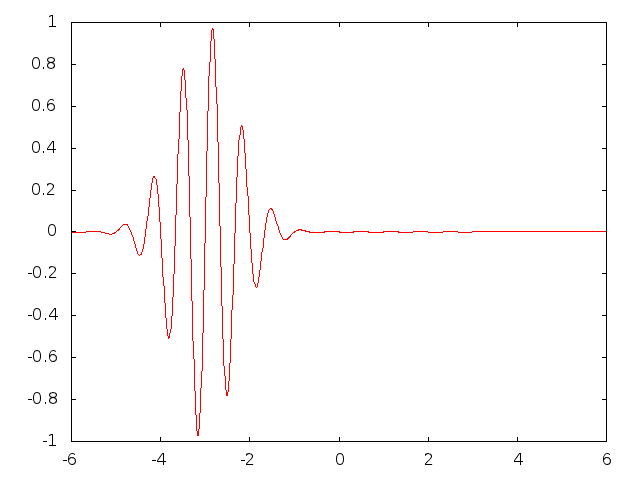
\includegraphics[width=0.9\linewidth]{../doc/manual/figs/wavepacket_0001.png}}
\end{center}

% !eslidecell

% !bpop highlight-red
Here we have a paragraph to pop up in red.
And a line more
% !epop

\shortinlinecomment{hpl 1}{ Here are some notes that can go to notes typesetting
in the slide environment. }{ Here are some notes }

% !bnotes
One can also have ordinary notes.
Over multiple lines.
% !enotes

% !split
\subsection{Scientific writing needs to address many new media}

% !bpop

\begin{itemize}
 \item Old days (1985-2005): mostly black-and-white documents aimed at printing

 \item Now: also color PDF, web pages, wikis - for paper, PC, iPad, ...

 \item {\LaTeX} writing may be very different from writing in other formats

 \item Main problem:
\begin{itemize}

    \item {\LaTeX} provide all sorts of fancy packages, but

    \item PDF in browsers has limited capabilities (design, navigation)
      compared to native HTML formats

\end{itemize}

\noindent
 \item Conclusion: We need more than {\LaTeX}
\end{itemize}

\noindent
% !epop

% !split
\subsection{Some math and computer code}

\[ f(x,y,t) = e^{-xt}\sin\pi y \]
Python implementation:

\bpycod
import numpy as np

def f(x, y, t):
    return np.exp(-x*t)*np.sin(np.pi*y)

class Fancy:
    def __init__(self):
        pass

    def __call__(self, x, y, t):
        return f(x, y, t)

f2 = Fancy()
\epycod

% !split
\subsection{Admon blocks}

Can use admons to simulate blocks:


\begin{graybox1admon}[Key PDE:]
This box has title and math in normal 90 percent font:
\[ \frac{\partial u}{\partial t} = \nabla^2 u \]
\end{graybox1admon}

% !bpop

\begin{graybox1admon}[]
Just some block with text and a conclusion that something is important.
This one pops up after the rest of the slide.
\end{graybox1admon}

% !epop


\begin{graybox1admon}[Warning.]
\vspace{0.5mm}\par\noindent
{\footnotesize Can use, e.g., a warning admon to have my own notes, preferably
inside preprocess/mako if statements to turn notes on and off.
This one is typeset in a small font and with the default
title (Warning) since no title is specified. \par}
\end{graybox1admon}

% ------------------- end of main content ---------------


% #ifdef PREAMBLE
\printindex

\end{document}
% #endif

